%-----------------------------------------------------------------------------------
%	PACKAGES AND OTHER DOCUMENT CONFIGURATIONS
%----------------------------------------------------------------------------------

\documentclass[11pt]{article}

\usepackage[top=2cm, bottom=3cm, left=2cm, right=2cm]{geometry}

\setlength{\parindent}{0in}

\newcommand{\Var}{\mathrm{Var}}

\newcommand{\Cov}{\mathrm{Cov}}

\newcommand{\plim}{\rightarrow_{p}}

\usepackage{amsmath, amsfonts}
\usepackage{graphicx}
\usepackage{pdfpages}
\usepackage{bm}
\usepackage{listings}
\usepackage{multirow,array}
\usepackage{enumerate}
\usepackage{bbm}


\usepackage[latin1]{inputenc}

\usepackage{amssymb}

\usepackage{mathrsfs}
\usepackage{float}
\usepackage{booktabs}
\usepackage{color}
\usepackage{rotating}
\usepackage{amsthm}
\usepackage{multirow,array}
\usepackage{caption}
\usepackage{url}


\DeclareMathOperator*{\argmax}{arg\,max}
\DeclareMathOperator*{\argmin}{arg\,min}



% Expectation symbol
\newcommand{\E}{\mathrm{E}}
\newcommand{\V}{\mathrm{V}}
\newcommand{\N}{\mathcal{N}}
\newcommand{\R}{\mathbb{R}} 

%----------------------------------------------------------------------------------
%	TITLE AND AUTHOR(S)
%----------------------------------------------------------------------------------
\title{Econ 675 Assignment 3} % The article title


\author{Nathan Mather\thanks{Shouts out to Ani  for the help with this. Could not have done it without you! } } % The article author(s) 

\date{\today} % An optional date to appear under the author(s)


%----------------------------------------------------------------------------------
\begin{document}
	
%------------------------------------------------------------------------------
%	TABLE OF CONTENTS & LISTS OF FIGURES AND TABLES
%------------------------------------------------------------------------------
\maketitle % Print the title/author/date block

\setcounter{tocdepth}{2} % Set the depth of the table of contents to show sections and subsections only

\tableofcontents % Print the table of contents


%-------------------------------------------------------------
% Question 1 
%-------------------------------------------------------------
\section{Question 1: Estimating Equations }

\subsection{Q1 Part 1}

To show that these are valid moment conditions we just need to show that they are all equal to zero. We start with the IPW condition 

$$ \E \left[ \psi_{IPW}(\bm{Z}_i;\theta_t(g)) \right] = \E \left[ \frac{D_i(t) \cdot g(Y_i(t))}{p_t(\bm{X}_i)} - \theta(g)  \right] = \E \left[ \E \left[\frac{D_i(t) \cdot g(Y_i(t))}{p_t(\bm{X}_i)} | \bm{X}_i \right]  \right] - \theta(g) 
$$

$$ = \E \left[ \frac{1}{p_t(\bm{X}_i)} \E \left[  D_i(t) \cdot g(Y_i(t))| \bm{X}_i \right]  \right] - \theta(g) 
$$

Now notice that 
$$ \E[ D_i(t) | \bm{X}_i] = Pr[D_i(t) = 1| \bm{X}_i ] = Pr[T_i = t| \bm{X}_i ] = p_t(\bm{X}_i)
$$

using this we get 
$$ \E \left[ \psi_{IPW}(\bm{Z}_i;\theta_t(g)) \right] = \E \left[ \E \left[g(Y_i(t))| \bm{X}_i \right]  \right] - \theta(g) =  \E \left[g(Y_i(t)) \right] - \theta(g) = 0 $$

Next we check $\psi_{RI1,t}$
$$\E[\psi_{RI1,t}(\bm{Z}_i;\theta_t(g))] = \E[e_t(g;\bm{X}_i)] - \theta_t(g) = \E[\E[g(Y_i(t))|\bm{X}_i]] - \theta_t(g) = \E[g(Y_i(t))] - \theta_t(g) =0 
$$

Next check $\psi_{RI2,t}$
$$ \E[\psi_{RI2,t}(\bm{Z}_i;\theta_t(g))] = \E \left[ \frac{D_i(t) \cdot e_t(g;\bm{X_i})}{p_t(\bm{X}_i)} \right] - \theta(g) = \E \left[ \E \left[ \frac{D_i(t) \cdot e_t(g;\bm{X_i})}{p_t(\bm{X}_i)} | \bm{X}_i \right] \right] - \theta(g) = \E[e_t(g;\bm{X}_i)] - \theta_t(g) = 0
$$

Finally we check $\psi_{DR,t}$

$$ \E[\psi_{DR,t}(\bm{Z}_i;\theta_t(g))] = \E \left[ \frac{D_i(t) \cdot g(Y_i(t))}{p_t(\bm{X}_i)} - \theta(g)  \right] - \E \left[ \frac{e_t(g;\bm{X}_i)}{p_t(\bm{X}_i)}  (D_i(t) - p_t(\bm{X}_i)) \right]
$$

This first terms are identical to the IPW condition so we need only check the following. 

$$  \E \left[ \frac{e_t(g;\bm{X}_i)}{p_t(\bm{X}_i)}  (D_i(t) - p_t(\bm{X}_i)) \right] =  \E \left[ \frac{e_t(g;\bm{X}_i)D_i(t)}{p_t(\bm{X}_i)}   - pe_t(g;\bm{X}_i) \right] =  \theta_t(g) -  \theta_t(g) =0 $$
So all functions are valid moment conditions

\subsection{Q1 Part 2}

The plug-in IPW estimator is 
$$
\hat{\theta}_{\texttt{IPW},t}(g) = \frac{1}{n}\sum_{i=1}^n\frac{D_i(t)g(Y_i)}{\hat p_t(\bm{X}_i)}
$$

 $\hat p_t(\bm{X}_i)$ is the estimated propensity score. Because this has multiple treatment levels we can estimate the propensity score with any suitable discrete choice model. For example the multinomial logit model. \\ 
 

The RD1 estimator is 
\begin{align*}
\hat{\theta}_{\texttt{RI1},t}(g) = \hat{\E}[e_t(g;\bm{X}_i)] =  \frac{1}{n}\sum_{i=1}^n \hat{\E}[g(Y_i(t))|\bm{X}_i] &=  \frac{1}{n}\sum_{i=1}^n \hat{\E}[g(Y_i(t))|\bm{X}_i, D_i(t)=1] \\
&= \frac{1}{n}\sum_{i=1}^n \hat{\E}[g(Y_i)|\bm{X}_i, D_i(t)=1],
\end{align*}
where the second last equality uses the ignorability assumption. We just need to decide how to estimate this last term. We could probably use NLS or some nonparametric methid.


The plug-in `hybrid' imputation estimator is 
\begin{align*}
\hat{\theta}_{\texttt{RI2},t}(g) &=  \frac{1}{n}\sum_{i=1}^n\frac{D_i(t)\widehat{\mu}_t(\bm{X}_i)}{\hat p_t(\bm{X}_i)}. 
\end{align*}

Finally, the plug-in doubly robust estimator is given by
\begin{align*}
\hat{\theta}_{\texttt{DR},t}(g) &= \frac{1}{n}\sum_{i=1}^n\frac{D_i(t)g(Y_i)}{\hat p_t(\bm{X}_i)}-\frac{1}{n}\sum_{i=1}^n\frac{\widehat{\mu}_t(\bm{X}_i)}{\hat p_t(\bm{X}_i)}(D_i(t) - \hat p_t(\bm{X}_i))\\
&=\frac{1}{n}\sum_{i=1}^n \left(\frac{D_i(t)(g(Y_i) - \widehat{\mu}_t(\bm{X}_i))}{\hat p_t(\bm{X}_i)} + \widehat{\mu}_t(\bm{X}_i) \right).
\end{align*}

As discussed in Abadie and Catteneo (2018), the relative performance of the above estimators depends on the features of the data generating process. In finite samples, IPW estimators become unstable when the propensity score approaches zero or one and regression imputation estimators may suffer from extrapolation biases. Doubly robust estimators include safeguards against bias caused by misspecification but impose additional specification choices that may affect the resulting estimate.

\subsection{Q1 Part 3}

Note that 
\begin{align*}
\sigma_t^2 = \V[Y_i(t)] = \E\left[Y_i(t) - \E[Y_i(t)]\right]^2
\end{align*}

Thus, we can estimate $\sigma_t^2$ using any of the Methods from 1.2, with $g(Y_i(t)) = \E\left[Y_i(t) - \E[Y_i(t)]\right]^2$. This would be a two-step estimator, since we would need to estimate $\E[Y_i(t)]$. To conduct the hypothesis test of $H_0: \sigma_t^2 = \sigma^2 \text{ } \forall t \in \mathcal{T}$ we would need to use an appropriate joint hypothesis testing procedure. One way to proceed would be test  $H_0: \sigma_t^2 - \sigma^2 =0 \text{ } \forall t \in \mathcal{T}$  and construct the vector $\widehat{\bm{\theta}}= (\hat \sigma^2_1-\sigma^2,...,\hat\sigma^2_T-\sigma^2)'$, and then show $\sqrt{n}(\widehat{\bm{\theta}}-\bm{\theta}_0) \to \N(0,V)$. Then, the Delta method implies $\sqrt{n}(||\widehat{\bm{\theta}}||^2-||\bm{\theta}_0||^2) \to \N(0,4\bm{\theta}_0'V\bm{\theta}_0)$. Note that under the null $\bm{\theta}_0=0$, so we can now conduct the hypothesis test $H_0: \bm{\theta}_0=0$ in the usual way, using an estimator for the asymptotic variance.


\subsection{Q1 Part 4}
No Thanks 


%------------------------------------------------------------------
% Question 2
%------------------------------------------------------------------

\section{Question 2: Estimating Average Treatment Effects}

A few things didn't run in R but it all went through in STATA. Results are below. I only did one table because making it is tedious but the code for both programs is in the appendix 

\begin{center}
	
			\centering
	
	\textbf{ATE}\par\medskip
	\scalebox{0.85}{
	% latex table generated in R 3.5.1 by xtable 1.8-3 package
% Sun Nov 11 21:25:22 2018
\begin{tabular}{llrrrrrrrr}
  \hline
statistic & specificaiton & estimate\_exp & std.error\_exp & CI\_L & CI\_U & estimate\_PSID & std.error\_PSID & CI\_L & CI\_U \\ 
  \hline
Mean Diff &  & 1794 & 670 & 479 & 3109 & -15204 & 656 & -16490 & -13919 \\ 
  OLS & a & 1582 & 659 & 291 & 2873 & 6302 & 1209 & 3932 & 8673 \\ 
  OLS & b & 1507 & 657 & 219 & 2795 & 4699 & 1027 & 2686 & 6712 \\ 
  OLS & c & 1501 & 663 & 202 & 2800 & 4284 & 1031 & 2263 & 6306 \\ 
  Reg. Impute & a & 1462 & 630 & 228 & 2697 & -11195 & 1741 & -14608 & -7782 \\ 
  Reg. Impute & b & 1454 & 631 & 218 & 2690 & -10398 & 3549 & -17355 & -3442 \\ 
  Reg. Impute & c & 1428 & 642 & 170 & 2685 & -11920 & 3498 & -18776 & -5065 \\ 
  IPW & a & 1537 & 630 & 303 & 2772 & -13507 & 2800 & -18996 & -8019 \\ 
  IPW & b & 1470 & 631 & 234 & 2706 & -7246 & 3550 & -14204 & -288 \\ 
  IPW & c & 1468 & 642 & 210 & 2726 & -7487 & 3499 & -14344 & -629 \\ 
  D. Robust & a & 1473 & 630 & 239 & 2707 & -13507 & 2800 & -18996 & -8019 \\ 
  D. Robust & b & 1451 & 631 & 215 & 2687 & -11419 & 3549 & -18376 & -4463 \\ 
  D. Robust & c & 1423 & 642 & 166 & 2682 & -12504 & 3498 & -19360 & -5649 \\ 
  N1 Match & a & 1829 & 780 & 302 & 3358 & -15619 & 1153 & -17880 & -13359 \\ 
  N1 Match & b & 1876 & 735 & 435 & 3316 & -9350 & 3975 & -17140 & -1559 \\ 
  N1 Match & c & 1672 & 726 & 248 & 3095 & -9560 & 4034 & -17467 & -1656 \\ 
  P Match & a & 1542 & 646 & 275 & 2808 & -15859 & 6750 & -29089 & -2629 \\ 
  P Match & b & 1489 & 765 & -12 & 2989 & 8646 & 15056 & -20863 & 38156 \\ 
  P Match & c & 1257 & 677 & -70 & 2584 & -9562 & 4034 & -17468 & 1657 \\ 
   \hline
\end{tabular}

}
\end{center}

\newpage

\begin{center}
	
	\centering
	
	\textbf{ATT}\par\medskip
	\scalebox{0.85}{
		% latex table generated in R 3.5.1 by xtable 1.8-3 package
% Sun Nov 11 21:30:53 2018
\begin{tabular}{llrrrrrrrr}
  \hline
statistic & specificaiton & estimate\_exp & std.error\_exp & CI\_L & CI\_U & estimate\_PSID & std.error\_PSID & CI\_L & CI\_U \\ 
  \hline
Mean Diff &  & 1794 & 670 & 479 & 3109 & -15204 & 656 & -16490 & -13919 \\ 
  OLS & a & 1582 & 659 & 291 & 2873 & 6302 & 1209 & 3932 & 8673 \\ 
  OLS & b & 1507 & 657 & 219 & 2795 & 4699 & 1027 & 2686 & 6712 \\ 
  OLS & c & 1501 & 663 & 202 & 2800 & 4284 & 1031 & 2263 & 6306 \\ 
  Reg. Impute & a & 1462 & 630 & 228 & 2697 & -11195 & 1741 & -14608 & -7782 \\ 
  Reg. Impute & b & 1454 & 631 & 218 & 2690 & -10398 & 3549 & -17355 & -3442 \\ 
  Reg. Impute & c & 1428 & 642 & 170 & 2685 & -11920 & 3498 & -18776 & -5065 \\ 
  IPW & a & 1537 & 630 & 303 & 2772 & -13507 & 2800 & -18996 & -8019 \\ 
  IPW & b & 1470 & 631 & 234 & 2706 & -7246 & 3550 & -14204 & -288 \\ 
  IPW & c & 1468 & 642 & 210 & 2726 & -7487 & 3499 & -14344 & -629 \\ 
  D. Robust & a & 1473 & 630 & 239 & 2707 & -13507 & 2800 & -18996 & -8019 \\ 
  D. Robust & b & 1451 & 631 & 215 & 2687 & -11419 & 3549 & -18376 & -4463 \\ 
  D. Robust & c & 1423 & 642 & 166 & 2682 & -12504 & 3498 & -19360 & -5649 \\ 
  N1 Match & a & 1829 & 780 & 302 & 3358 & -15619 & 1153 & -17880 & -13359 \\ 
  N1 Match & b & 1876 & 735 & 435 & 3316 & -9350 & 3975 & -17140 & -1559 \\ 
  N1 Match & c & 1672 & 726 & 248 & 3095 & -9560 & 4034 & -17467 & -1656 \\ 
  P Match & a & 1542 & 646 & 275 & 2808 & -15859 & 6750 & -29089 & -2629 \\ 
  P Match & b & 1489 & 765 & -12 & 2989 & 8646 & 15056 & -20863 & 38156 \\ 
  P Match & c & 1257 & 677 & -70 & 2584 & -9562 & 4034 & -17468 & 1657 \\ 
   \hline
\end{tabular}

	}
\end{center}


%------------------------------------------------------------------
% Question 
%------------------------------------------------------------------

\section{Question 3: Post-model Seelction Inference}


\begin{center}
	
	\centering
	
	\textbf{Summary Stats}\par\medskip
	\scalebox{0.85}{
		% latex table generated in R 3.5.1 by xtable 1.8-3 package
% Sun Nov 11 23:00:22 2018
\begin{tabular}{lrrrrrr}
  \hline
estimator & Min. & 1st Qu. & Median & Mean & 3rd Qu. & Max. \\ 
  \hline
i & -0.50 & 0.32 & 0.52 & 0.51 & 0.71 & 1.32 \\ 
  ii & 0.77 & 1.26 & 1.36 & 1.36 & 1.47 & 1.88 \\ 
  iii & -0.50 & 0.32 & 0.52 & 0.54 & 0.72 & 1.66 \\ 
   \hline
\end{tabular}

	}
\end{center}

\begin{center}
	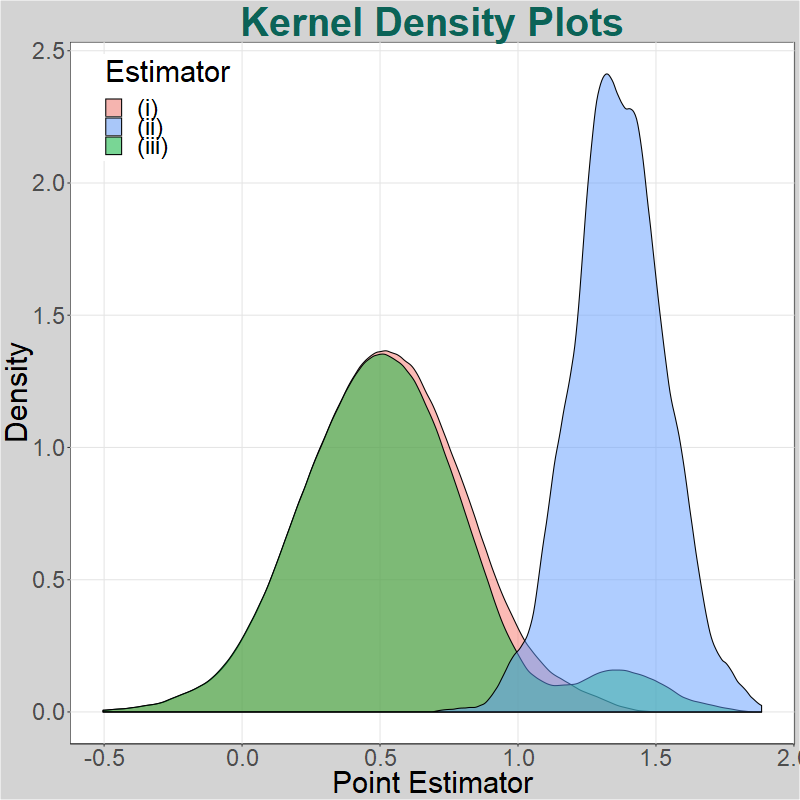
\includegraphics[width=.8\linewidth]{q4_den.png}
	
\end{center}

\subsection{Q3 Part 2}

\begin{center}
	
	\centering
	
	\textbf{Coverage Rates }\par\medskip
	\scalebox{0.85}{
		% latex table generated in R 3.5.1 by xtable 1.8-3 package
% Sun Nov 11 23:00:22 2018
\begin{tabular}{lrrrrrr}
  \hline
estimator & Min. & 1st Qu. & Median & Mean & 3rd Qu. & Max. \\ 
  \hline
i & -0.50 & 0.32 & 0.52 & 0.51 & 0.71 & 1.32 \\ 
  ii & 0.77 & 1.26 & 1.36 & 1.36 & 1.47 & 1.88 \\ 
  iii & -0.50 & 0.32 & 0.52 & 0.54 & 0.72 & 1.66 \\ 
   \hline
\end{tabular}

	}
\end{center}
%------------------------------------------------------------------------------------------------
% APPENDIX 
%------------------------------------------------------------------------------------------------

\section{Appendix}
\subsection{R Code}

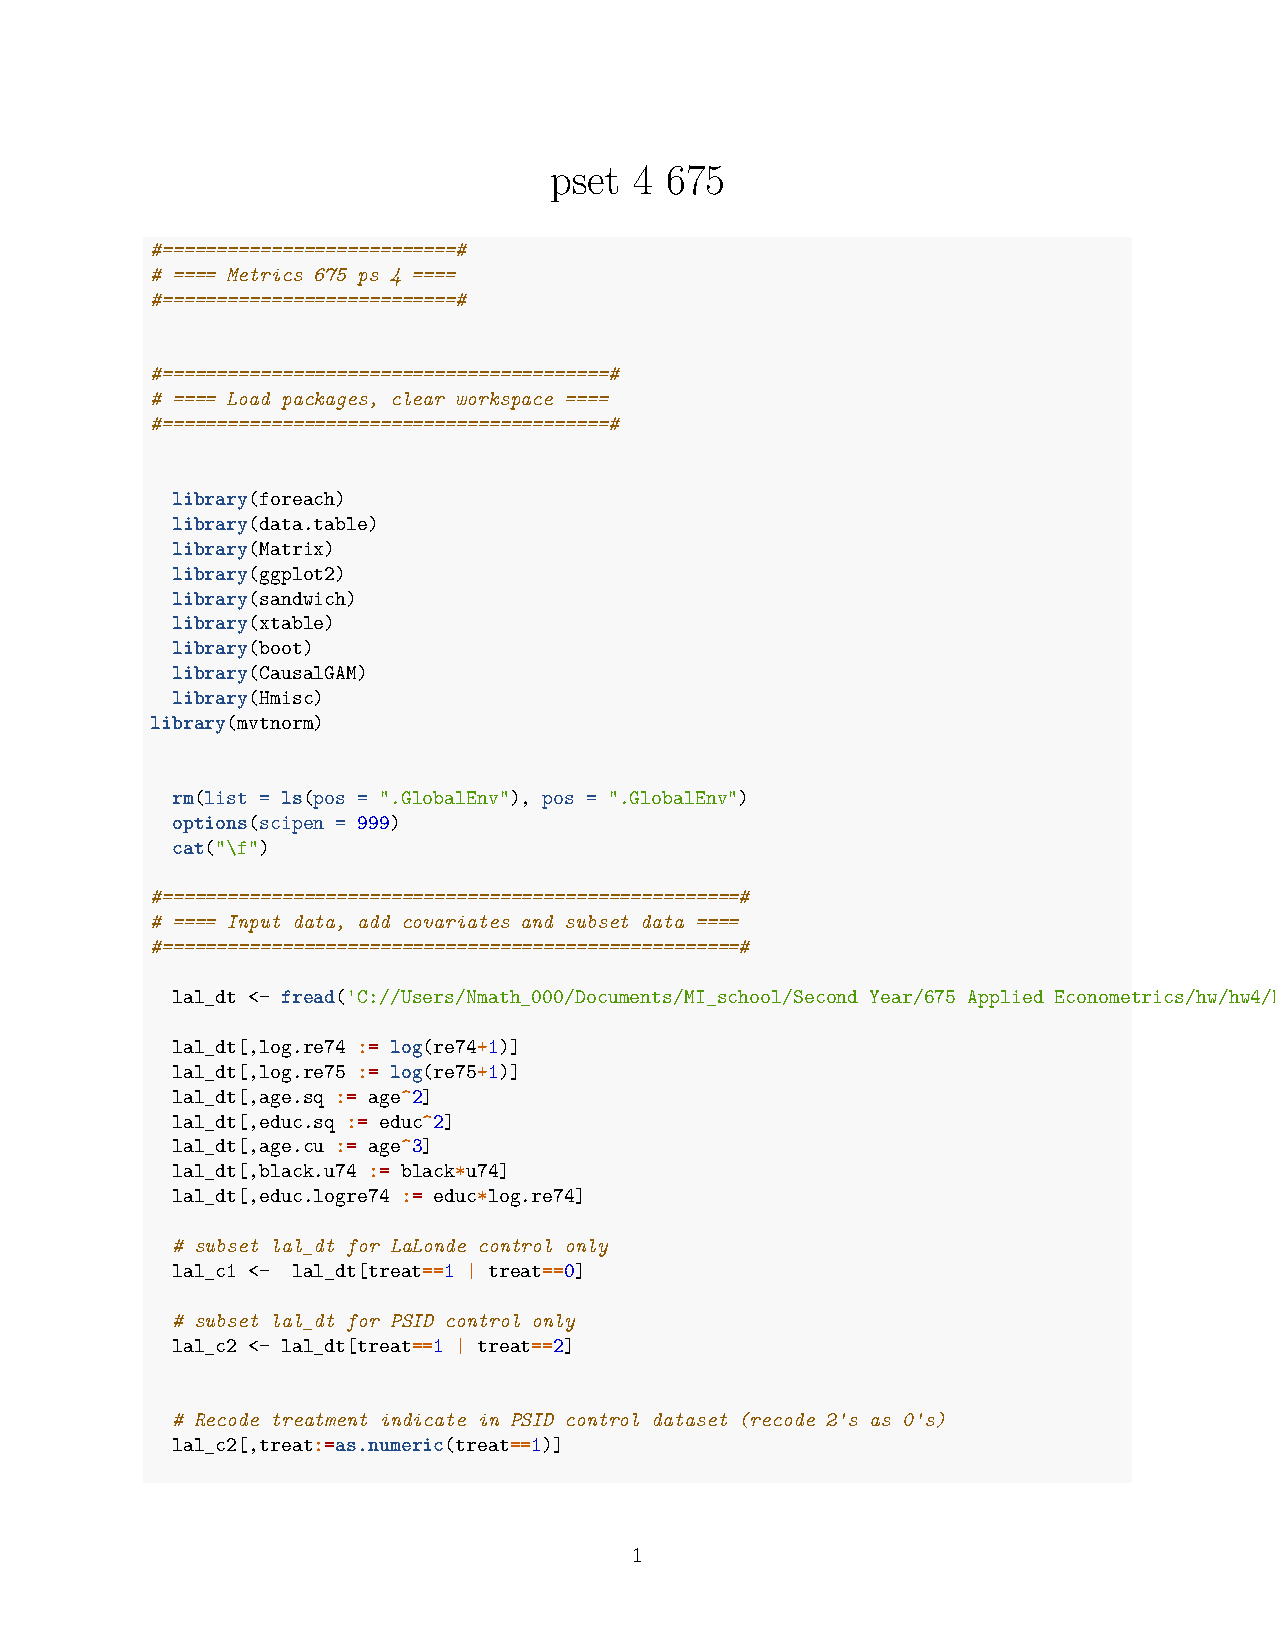
\includepdf[page=-]{assignment_4_r_code_pdf.pdf}

\subsection{STATA Code}
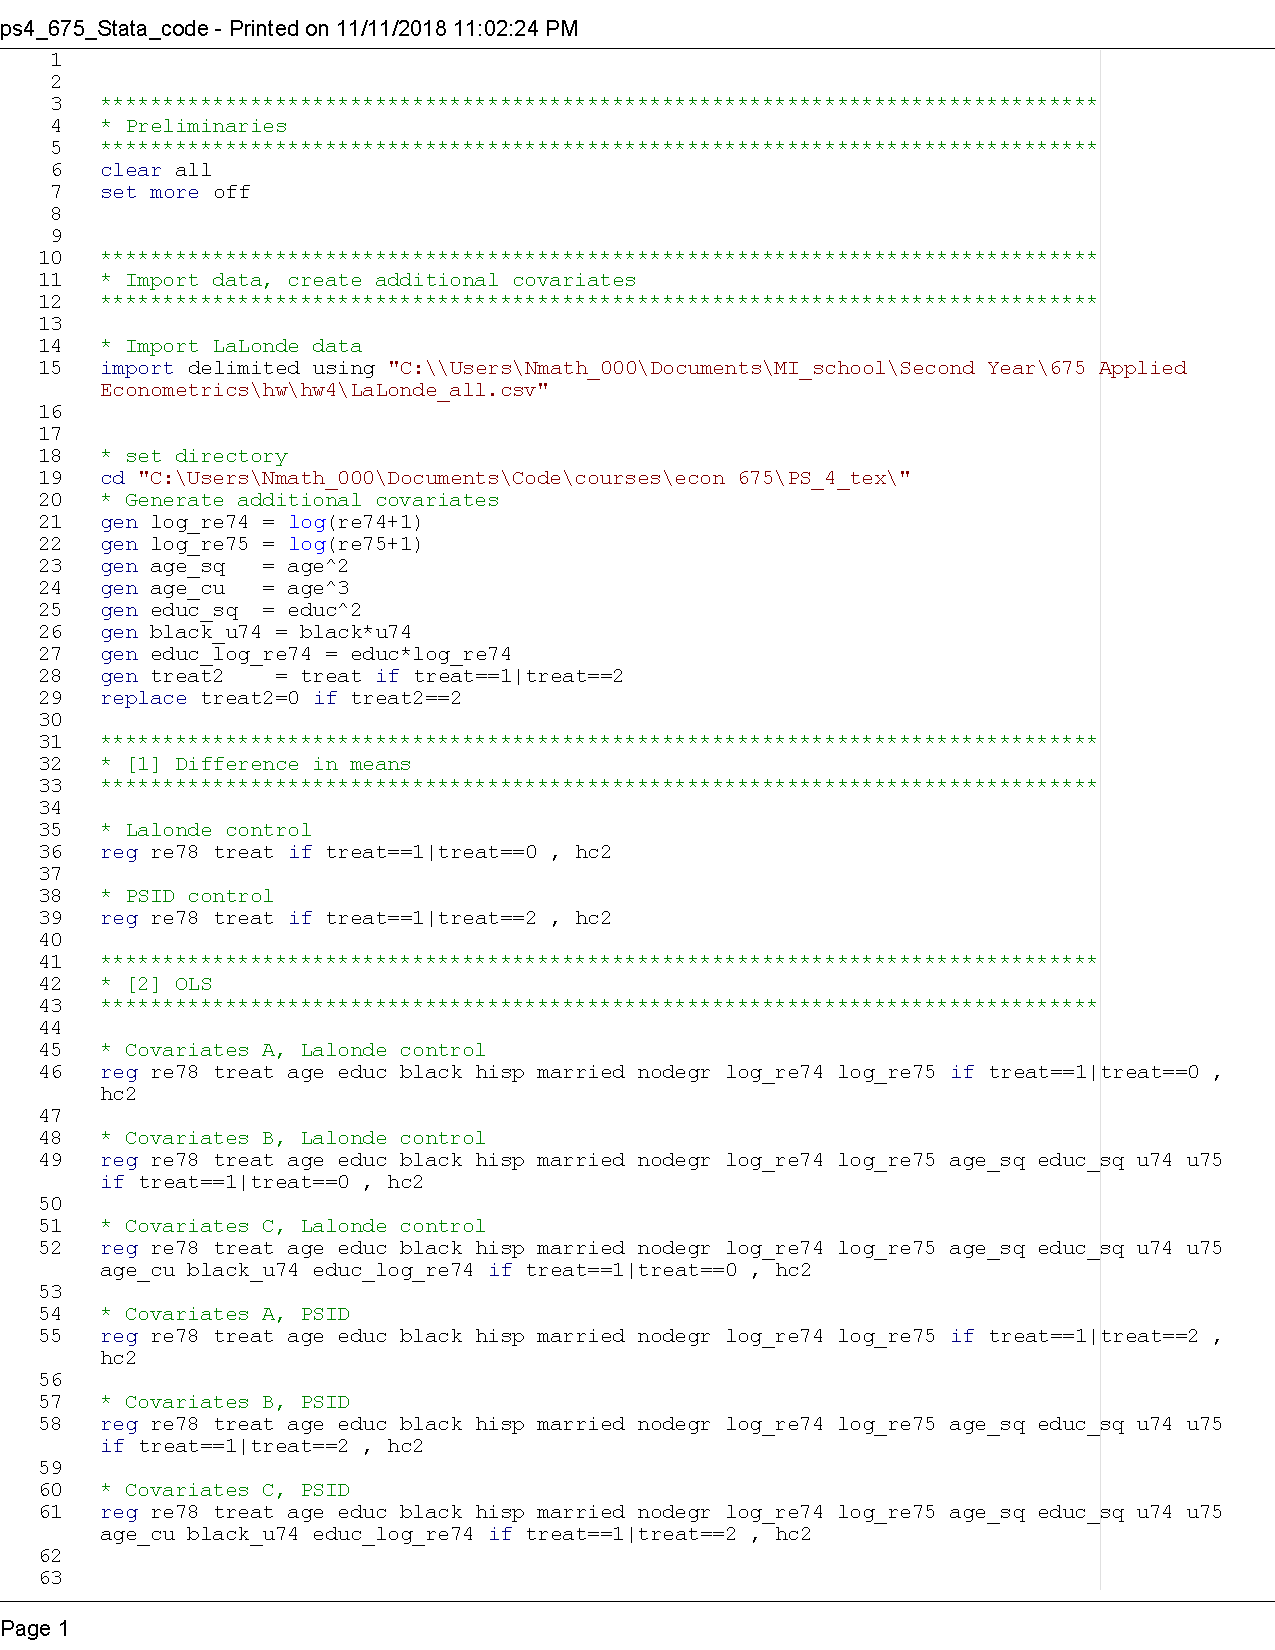
\includepdf[page=-]{ps_4_675_stata_code.pdf}

%------------------------------------------------
% end doc
%------------------------------------------------
\end{document}
